\section{Формирование наград для предотвращения взлома наград в обучении
 с подкреплением на основе человеческой обратной связи}


\subsection{Ключевые идеи}

Авторы формулируют два принципа эффективного преобразования награды в RLHF:

\begin{enumerate}
    \item Награда должна быть ограничена~-- чтобы уменьшить дисперсию возврата и 
        стабилизировать обучение критика.
    \item Награда должна обладать быстрым ростом около нуля и постепенным 
        насыщением~-- чтобы обеспечить быстрые начальные градиенты и стабильное 
        долгосрочное обучение.
\end{enumerate}

Метод \emph{Preference As Reward (PAR)} удовлетворяет обоим принципам и 
интерпретируется как модель предпочтений Брэдли--Терри: сигмоида от разницы 
наград задаёт вероятность того, что ответ политики предпочтительнее ссылочного.


\subsection{Математическое описание метода}

Основой метода PAR является преобразование прокси-награды $r = r_\varphi(x,y)$
с использованием награды ссылочного ответа 
$r_{\mathrm{ref}} = r_\varphi(x, y_{\mathrm{ref}})$.

\begin{definition}
    \label{def:centered_reward_short}
    \emph{Центрированная награда} определяется как
    \begin{equation}
        r_{\mathrm{center}} = r - r_{\mathrm{ref}}.
    \end{equation}
\end{definition}

Идея PAR состоит в том, чтобы использовать вероятность того, что ответ политики 
предпочтительнее ссылочного. Сигмоида от разности наград интерпретируется 
как скрытая вероятность предпочтения
в смысле модели Брэдли--Терри:

\begin{equation}
\label{eq:bt-preference}
    P_\varphi( y \succ y_{\mathrm{ref}} \mid x )
    =
    \sigma\!\left( r - r_{\mathrm{ref}} \right),
    \qquad 
    \sigma(z)=\frac{1}{1+e^{-z}} .
\end{equation}

\begin{definition}
    \label{def:par_short}
    \emph{Награда PAR} для обучения с подкреплением определяется как
    \begin{equation}
        r_{\mathrm{RL}}
        =
        \frac{1}{M}
        \sum_{m=1}^M
        \sigma\!\left(
            r - r_{\mathrm{ref}}^{(m)}
        \right).
    \end{equation}
\end{definition}

Таким образом, RL-награда становится ограниченной
$ 0 < r_{\mathrm{RL}} < 1, $ а её рост максимален при небольших отклонениях 
политики от ссылочной. Это удовлетворяет двум принципам, сформулированным авторами:

\begin{itemize}
    \item ограниченность награды~-- снижает дисперсию возврата и стабилизирует 
    критика;
    \item быстрый рост при $r \approx r_{\mathrm{ref}}$ и плавное насыщение 
    при больших значениях.
\end{itemize}

Эти свойства обеспечивают устойчивое обучение и предотвращают
изменение прокси-награды.


\subsection{Математическое описание метода}

Метод \emph{Preference As Reward (PAR)} основан на преобразовании прокси-награды 
$r = r_\varphi(x,y)$ путём сравнения ответа политики с ответом ссылочной политики 
$y_{\mathrm{ref}} \sim \pi_{\mathrm{ref}}(\,\cdot\mid x)$.
    
Центрированная награда определяется как
    \begin{equation}
        r_{\mathrm{center}} = r - r_{\mathrm{ref}},
        \qquad 
        r_{\mathrm{ref}} = r_\varphi(x, y_{\mathrm{ref}}).
    \end{equation}

Сигмоида от центрированной награды интерпретируется как вероятность того,
что ответ политики предпочтительнее ссылочного в смысле скрытой модели предпочтений:
\begin{equation}
    P_\varphi\!\left(y \succ y_{\mathrm{ref}} \mid x\right)
    =
    \sigma\!\left( r - r_{\mathrm{ref}} \right),
    \qquad 
    \sigma(z)=\frac{1}{1+e^{-z}} .
\end{equation}

Награда PAR при использовании $M$ ссылочных ответов задаётся как
    \begin{equation}
        r_{\mathrm{RL}}
        =
        \frac{1}{M}\sum_{m=1}^M
        \sigma\!\left(
            r - r_{\mathrm{ref}}^{(m)}
        \right).
    \end{equation}

Таким образом, награда PAR удовлетворяет двум принципам:
\begin{itemize}
    \item награда ограничена ($0 < r_{\mathrm{RL}} < 1$), что снижает дисперсию 
    возврата;
    \item кривая роста имеет максимальный градиент вблизи $r = r_{\mathrm{ref}}$ 
    и плавно насыщается, что предотвращает переразгон прокси-награды и 
    разрушение политики.
\end{itemize}

На рисунке ниже показано, что обучение PPO с использованием PAR обеспечивает 
значительно более стабильные значения потерь политики и критика по сравнению 
со стандартным вариантом.

\begin{figure}[h]
    \centering
    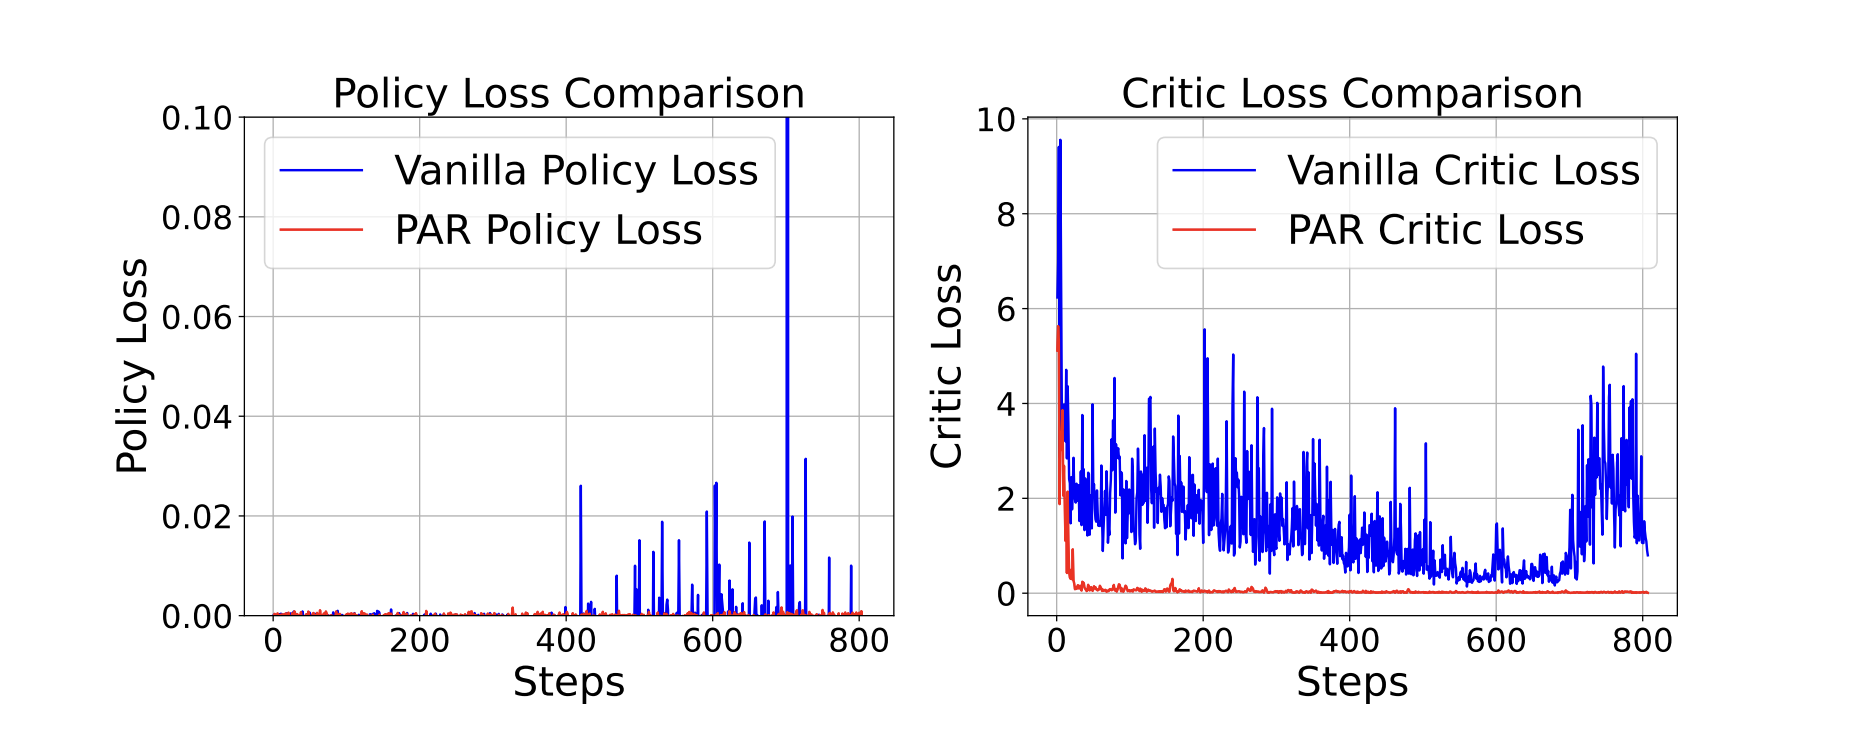
\includegraphics[width=0.9\linewidth]{images/par_losses.png}
    \caption{
        Сравнение кривых потерь политики и критика при обучении PPO:
        метод PAR демонстрирует существенно больший уровень стабильности.
        Данная устойчивость обусловлена ограниченностью награды PAR.
    }
    \label{fig:par_losses}
\end{figure}

\subsection{Наборы данных}

В работе используются два набора данных предпочтений, необходимых для обучения 
модели награды и последующего обучения политики.

\begin{itemize}

    \item \emph{Ultrafeedback-Binarized} (см.~\cite{cui2023ultrafeedback})~--  
    набор бинарных предпочтений, где для каждого запроса даны два ответа
    и указано, какой из них является предпочтительным.  

    \item \emph{HH-RLHF Helpful Base} (см.~\cite{bai2022training})~--  
    подкорпус человеческих предпочтений, созданный для обучения 
    ''полезных'' моделей. Каждое наблюдение содержит выбранный и 
    отклонённый ответ на один и тот же запрос.

\end{itemize}

\subsection{Метрики}

\begin{itemize}
    \item \emph{Прокси-награда}~-- средняя награда от модели награды.
    \item \emph{Winrate}~-- процент побед модели над SFT-базой; оценивался 
    моделью DeepSeek-V3.
    \item \emph{AlpacaEval 2.0}~-- контролируемая и неконтролируемая доля 
    побед \cite{li2023alpacaeval}.
    \item \emph{MT-Bench}~-- оценки первого и второго хода диалога \cite{zheng2023judging}.
\end{itemize}

\subsection{Модели}

В работе используются языковые модели различного масштаба, которые 
служат основой для обучения политики, модели награды и оценивания качества.

\begin{itemize}

    \item \emph{Gemma-2B} (см.~\cite{google2024gemma})~--  
    компактная трансформерная модель с 2 млрд параметров.  
    В работе она используется как базовая модель и как архитектура для 
    дальнейшего дообучения: сперва для обучения SFT-модели, затем для политики 
    и модели награды.

    \item \emph{Llama~3--8B} (см.~\cite{meta2024llama3})~--  
    модель с 8 млрд параметров, обеспечивающая более высокую 
    выразительность. Она служит второй тестовой архитектурой, позволяя оценить 
    переносимость метода PAR на модели большего масштаба.

    \item \emph{DeepSeek-V3} (см.~\cite{deepseek2024v3})~--  
    модель-оценщик, применяемая для автоматического сравнения ответов 
    и расчёта метрики winrate. Она заменяет человеческих аннотаторов при 
    контроле качества модели в ходе обучения.

\end{itemize}
